\documentclass{article}
\usepackage{amsmath, amssymb}
\usepackage[margin=1in]{geometry}
\usepackage{setspace}
\usepackage{graphicx}
\usepackage{multicol}
\usepackage[backend=bibtex]{biblatex}

\addbibresource{mbib.bib}

\doublespacing

\title{The R\"{o}ssler System}
\author{Steven Rosendahl}
\date{}

\begin{document}
\maketitle

In 1976, Otto R\"{o}ssler proposed a system of nonlinear ordinary differential equations that illustrated the simplest possible strange attractor. An attractor is a set of values towards which a system moves when initial conditions are \textit{near} the attractor; to call an attractor \textit{strange} means that the attractor exhibits fractal behavior. Often, strange attractors are associated with chaotic systems. R\"{o}ssler's strange attractor is a chaotic attractor that solves his proposed system
\begin{align}
	f(x,y,z) = \dot{x} & = -y-z     \\
	g(x,y,z) = \dot{y} & = x+ay     \\
	h(x,y,z) = \dot{z} & = b+z(x-c)
\end{align}
where $a,b,$ and $c$ are arbitrary values. R\"{o}ssler studied the effects that small (i.e. less than 1) $a$ and $b$ paired with a relatively large $c$ had on the system's chaotic behavior. One such plot is shown in figure \ref{fig:3dsys_01}.

We first want to analyze the stability of the critical points of the system. The Jacobian for this system can be found by constructing a matrix of partial derivatives for $f,g,$ and $h$.
\[
	J(x,y,z)=
	\left[
	\begin{array}{c c c}
		\frac{\partial f}{\partial x} & \frac{\partial f}{\partial y} & \frac{\partial f}{\partial z} \\
		\frac{\partial g}{\partial x} & \frac{\partial g}{\partial y} & \frac{\partial g}{\partial z} \\
		\frac{\partial h}{\partial x} & \frac{\partial h}{\partial y} & \frac{\partial h}{\partial z} \\
	\end{array}
	\right]
	=
	\left[
	\begin{array}{c c c}
		0 & -1 & -1  \\
		1 & a  & 0   \\
		z & 0  & x-c
	\end{array}
	\right].
\]
We now need to find the critical points of the system. We can accomplish this by solving $f=0,g=0,$ and $h=0$. Through the use of Mathematica's \texttt{Solve} command, we get
\begin{center}
	\texttt{Solve[f[x, y, z] == 0 \&\& g[x, y, z] == 0 \&\& h[x, y, z] == 0, \{x, y, z\}]}
\end{center}
\begin{gather}
	\left[
	x=\frac{1}{2}\left(c-\sqrt{c^{2}-4ab}\right),
	y=\frac{1}{2}\left(\frac{\sqrt{c^{2}-4ab}}{a}-\frac{c}{a}\right),
	z=\frac{c-\sqrt{c^{2}-4ab}}{2a}
	\right]\label{eq:csln1}\\
	\left[
	x=\frac{1}{2}\left(c+\sqrt{c^{2}-4ab}\right),
	y=\frac{1}{2}\left(-\frac{\sqrt{c^{2}-4ab}}{a}-\frac{c}{a}\right),
	z=\frac{c+\sqrt{c^{2}-4ab}}{2a}
	\right]\label{eq:csln2}.
\end{gather}

R\"{o}ssler's analysis focused on the behavior of the system for small $a$ and $b$. For simplicity, we can consider the solutions to (\ref{eq:csln1}) and (\ref{eq:csln2}) for very small $a$ and $b$. We now have
\begin{gather}
	\left[
	x=0,
	y=0,
	z=0
	\right]\label{eq:csln1sm}\\
	\left[
	x=c,
	y=-\frac{c}{a},
	z=\frac{c}{a}
	\right]\label{eq:csln2sm}.
\end{gather}
To find the behavior around the critical points given by (\ref{eq:csln1sm}), we evaluate the Jacobian at the appropriate points and find the eigenvalues of the system.
\[
	|J(0,0,0)-\lambda I| =
	\left|
	\left[
	\begin{array}{c c c}
		-\lambda & -1       & -1         \\
		1        & -\lambda & 0          \\
		0        & 0        & -c-\lambda
	\end{array}
	\right]
	\right| =
	(c-\lambda)(\lambda + 1)^{2}=0.
\]
Hence, the system has three eigenvalues: $\lambda=-i, \lambda=-i,$ and $\lambda = -c$ (we will assume here that $c > 1$). This implies that the system has an unstable focus node at the origin \cite{equilibria}. Figure \ref{fig:plot_cuts} shows various cuts of the system for various $z$ values; the system spirals in the $x-y$ plane, while moving towards and then away from the origin as $z$ moves from $-\infty$ to $\infty$. We can solve this linearized system by looking at the equation
\[
	\mathbf{\dot{x}} =
	\left[
	\begin{array}{c c c}
		0 & -1 & -1 \\
		1 & 0  & 0  \\
		0 & 0  & -c
	\end{array}
	\right]
	\mathbf{x}.
\]
Since we've already found the eigenvalues of the system, we can find the eigenvectors immediately.

\begin{minipage}{0.3\textwidth}
	\begin{gather*}
		\text{\underline{$\lambda=-i$}}\\
		\mathbf{\lambda_{1}}=\left[
		\begin{array}{c}
			-i \\
			1  \\
			0
		\end{array}
		\right].
	\end{gather*}
\end{minipage}
\begin{minipage}{0.3\textwidth}
	\begin{gather*}
		\text{\underline{$\lambda=i$}}\\
		\mathbf{\lambda_{2}}=\left[
		\begin{array}{c}
			i \\
			1 \\
			0
		\end{array}
		\right].
	\end{gather*}
\end{minipage}
\begin{minipage}{0.3\textwidth}
	\begin{gather*}
		\text{\underline{$\lambda=-c$}}\\
		\mathbf{\lambda_{3}}=\left[
		\begin{array}{c}
			\frac{c}{1+c^{2}}  \\
			-\frac{1}{1+c^{2}} \\
			1
		\end{array}
		\right].
	\end{gather*}
\end{minipage}

\noindent\\
\noindent Letting $\mathbf{\gamma}$ stand in for our constants, we get
\[
	\mathbf{x}(t) =
	\gamma_{1}e^{-it}\left[
	\begin{array}{c}
		-i \\
		1  \\
		0
	\end{array}
	\right] +
	\gamma_{2}e^{it}
	\left[
	\begin{array}{c}
		i \\
		1 \\
		0
	\end{array}
	\right] +
	\gamma_{3}e^{-ct}\left[
	\begin{array}{c}
		\frac{c}{1+c^{2}}  \\
		-\frac{1}{1+c^{2}} \\
		1
	\end{array}
	\right].
\]
Note that we choose to leave the $e^{it}$ in this form, since \textbf{${\lambda_{1}}$} and $\mathbf{\lambda_{2}}$ are linearly independent of each other. Figure \ref{fig:zero_sln} shows the behavior of this linearized system with two different sets of initial conditions. If we compare this to figure \ref{fig:3dsys_02}, we see similar behavior in the area of the graph with large $z$ values.

This represents only one of the equilibrium points of the system, however. We now need to analyze the linearized system near (\ref{eq:csln2sm}). In this case, we cannot let $a$ tend towards zero as we did in (\ref{eq:csln1sm}) since our roots rely on division by $a$.
\[
	\left|J\left(c,-\frac{c}{a},\frac{c}{a}\right) -\lambda I\right| =
	\left|
	\left[
	\begin{array}{c c c}
		-\lambda    & -1          & -1       \\
		1           & a - \lambda & 0        \\
		\frac{c}{a} & 0           & -\lambda
	\end{array}
	\right]
	\right| =
	\frac{ ac - a\lambda - c\lambda + a^{2}\lambda^{2} -a\lambda^{3}}{a}.
\]
Setting the determinant to $0$ and solving in Mathematica yields three distinct (and incredibly verbose) eigenvalues with $\lambda_{1}\in\mathbb{R}$ the other two complex conjugates of each other. Such behavior lends itself towards what is known as a \textit{saddle focus}, which is always unstable \cite{equilibria}. Figure \ref{fig:3dsys_02} displays the behavior of both equilibrium points. The spiral behavior can be seen in the $x-y$ plane, and the saddle behavior can be seen predominantly in the $z-x$ plane.

Again, we can solve the linearized system and analyze the behavior as we did with the system centered around $(0,0,0)$. Due to the complexity of the eigenvalues of this system, we let Mathematica determine the behavior. The command
\begin{center}
	\texttt{Eigenvectors[jcbn[x, y, z] /. \{x -> c, y -> -(c/a), z -> (c/a)\}]}
\end{center}
yields an unfriendly expression involving the \texttt{Root} command; in this case we will want to give concrete values to $c$ and $a$. Figure \ref{fig:3dsys_02} involves the behavior of the system at $a=0.14$ and $c=8.8$, so we will examine the resulting eigenvalues at those points.
\begin{center}
	\texttt{Eigenvectors[jcbn[x, y, z] /. \{x -> c, y -> -(c/a), z -> (c/a)\}]/.\{a -> 0.14, c -> 8.8\}}
\end{center}
results in the following three eigenvectors:

\begin{minipage}{0.3\textwidth}
	\begin{gather*}
		% \text{\underline{$\lambda=-i$}}\\
		\mathbf{\lambda_{1}}=\left[
		\begin{array}{c}
			-0.0022 \\
			-1.0003 \\
			1.0000
		\end{array}
		\right]
	\end{gather*}
\end{minipage}
\begin{minipage}{0.3\textwidth}
	\begin{gather*}
		% \text{\underline{$\lambda=i$}}\\
		\mathbf{\lambda_{2}}=\left[
		\begin{array}{c}
			0.0000174 - 0.12713i \\
			0.0159 + 0.00028i    \\
			1
		\end{array}
		\right]
	\end{gather*}
\end{minipage}
\begin{minipage}{0.3\textwidth}
	\begin{gather*}
		% \text{\underline{$\lambda=-c$}}\\
		\mathbf{\lambda_{3}}=\left[
		\begin{array}{c}
			0.0000174 - 0.12713i \\
			0.0159 + 0.00028i    \\
			1
		\end{array}
		\right].
	\end{gather*}
\end{minipage}

\noindent\\
\noindent We now have enough to for a general solution with $\mathbf{\gamma}$ in place of our constants.
\begin{gather*}
	\mathbf{x}(t) =
	\gamma_{1}e^{0.138t}\left[
	\begin{array}{c}
		-0.0022 \\
		-1.0003 \\
		1
	\end{array}
	\right] +
	\gamma_{2}e^{(0.00109-7.99i)t}\left[
	\begin{array}{c}
		0.0000174 - 0.12713i \\
		0.0159 + 0.00028i    \\
		1
	\end{array}
	\right] +\\
	\gamma_{3}e^{(0.00109+7.99i)t}\left[
	\begin{array}{c}
		0.0000174 + 0.12713i \\
		0.0159 - 0.00028i    \\
		1
	\end{array}
	\right].
\end{gather*}
Figure \ref{fig:nzero_sln} displays two parametric plots of the solution curves for different initial values. The curves exhibit a center-like behavior that looks like a spring. We can compare this to the actual curve seen in \ref{fig:3dsys_02}. This behavior is seen in the purple spiral in the $x-y$ plane of the graph.

We now know that both equilibrium points are unstable when we ignore $a$ and $b$ in comparison to $c$. In fact, it turns out that this stability is preserved even when we reintroduce $a$ and $b$ back into the system. Figure \ref{fig:raw_ev} shows us what one of the raw eigenvalues looks like, according to Mathematica. The three eigenvalues resulting from the unsimplified system still exhibit the saddle focus behavior that we saw when we allowed $a$ and $b$ to drift towards zero. We now want to turn our attention towards the actions of the system when we change the values for $a$, $b$, and $c$.

Attractors are often associated with chaotic systems; as such, we will now examine various bifurcations on the R\"{o}ssler system. We have three variables that contribute to the chaos of the system: $a$, $b$, and $c$. R\"{o}ssler analyzed the system for relatively small $a$ and $b$, and we analyzed the stability of critical points when we neglected $a$ and $b$. We will first analyze the effect that small changes to $a$ have on the system.

The $a$ parameter affects our $g(x,y,z)$. For simplicity, we notice that $g$ is only dependent on $x$ and $y$, so we will let $g(x,y,z)=\gamma(x,y)$.

\newpage
\clearpage
\section*{Plots and Graphics}
\begin{figure}[h]
	\centering
	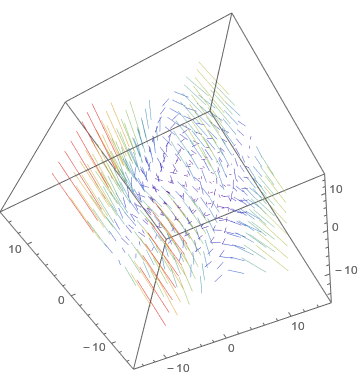
\includegraphics[scale=0.5]{vp_01.png}
	\caption{The R\"{o}ssler system with $a=0.2$, $b=0.1$, and $c=2.3$}
	\label{fig:3dsys_01}
\end{figure}

\begin{figure}[h]
	\centering
	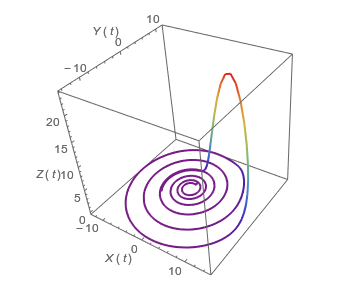
\includegraphics[scale=0.7]{attractor_a0p14_b0p2_c8p8}
	\caption{The R\"{o}ssler attractor with $a=0.14$, $b=0.2$, and $c=8.8$, courtesy of \cite{rossler_wf}}
	\label{fig:3dsys_02}
\end{figure}

\begin{figure}[h]
	\centering
	\begin{tabular}{c c}
		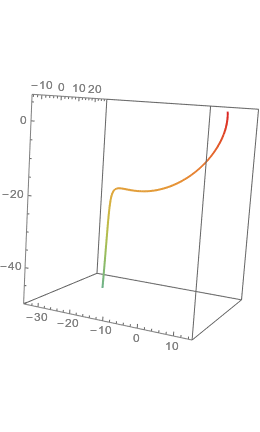
\includegraphics[scale=0.5]{gen_sln_01_01} & 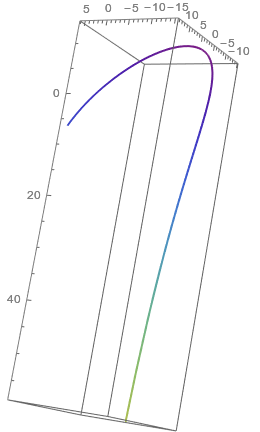
\includegraphics[scale=0.5]{gen_sln_01_02} \\
		$\gamma_{1}=-0.7$                          & $\gamma_{1}=-0.7$                          \\
		$\gamma_{2}=-0.7$                          & $\gamma_{2}=-0.7$                          \\
		$\gamma_{3}=-1$                            & $\gamma_{3}=1$                             \\
	\end{tabular}
	\caption{Two parametric plots for the linearized system around $(0,0,0)$ with different initial values}
	\label{fig:zero_sln}
\end{figure}

\begin{figure}[h]
	\centering
	\begin{tabular}{l r}
		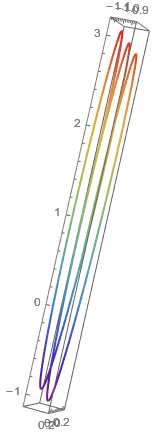
\includegraphics[scale=0.5]{gen_sln_02_01} & 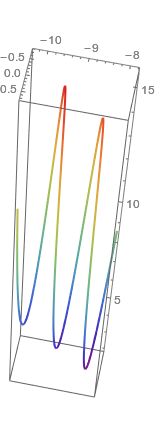
\includegraphics[scale=0.5]{gen_sln_02_02} \\
		$\gamma_{1}=1$                             & $\gamma_{1}=9$                             \\
		$\gamma_{2}=1$                             & $\gamma_{2}=-3$                             \\
		$\gamma_{3}=1$                            & $\gamma_{3}=-3$                             \\
	\end{tabular}
	\caption{Two parametric plots for the linearized system around $(c,-\frac{c}{a}, \frac{c}{a})$ with different initial values}
	\label{fig:nzero_sln}
\end{figure}

\begin{figure}[h]
	\centering
	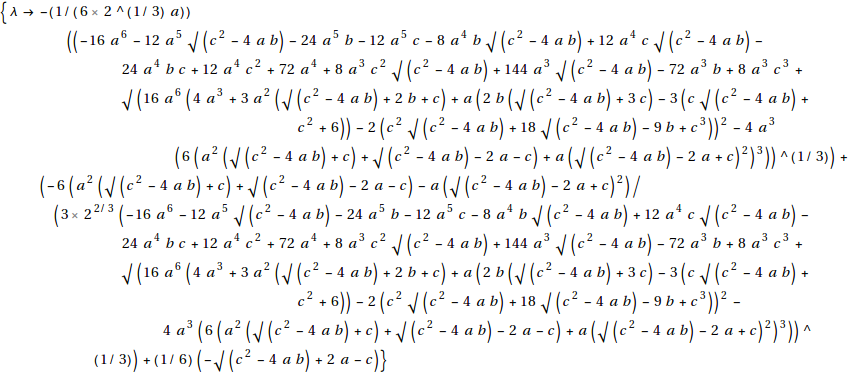
\includegraphics[scale=0.5]{messy_output}
	\begin{gather*}
		\{l\to -4.98425\}\\
		\{l\to 0.0961307\, -0.995341 i\}\\
		\{l\to 0.0961307\, +0.995341 i\}
	\end{gather*}
	\caption{Example of one raw eigenvalue and its corresponding evaluation at $a=0.2$, $b=0.2$, and $c=0.2$.}
	\label{fig:raw_ev}
\end{figure}

\begin{figure}[h]
	\centering
	\begin{tabular}{c c}
		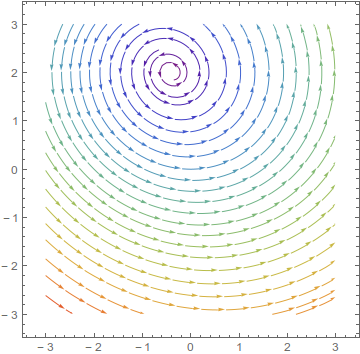
\includegraphics[scale=0.5]{spz-2} & 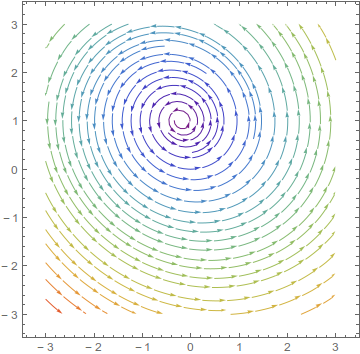
\includegraphics[scale=0.5]{spz-1} \\
		$z=-2$                             & $z=-1$                             \\
		\multicolumn{2}{c}{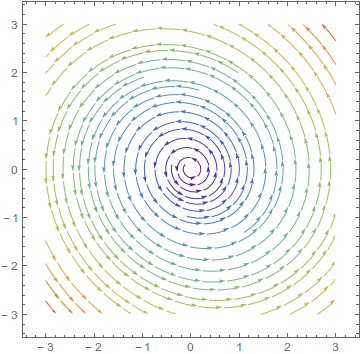
\includegraphics[scale=0.5]{spz0}}\\
		\multicolumn{2}{c}{$z=0$}\\
		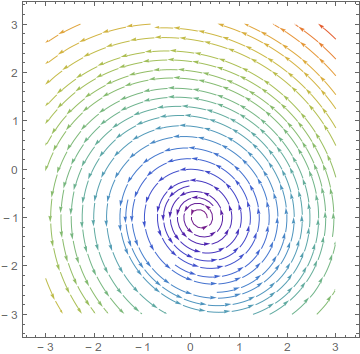
\includegraphics[scale=0.5]{spz1}  & 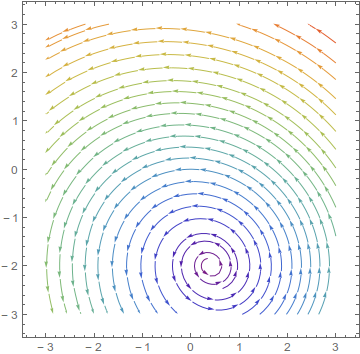
\includegraphics[scale=0.5]{spz2}  \\
		$z=1$                              & $z=2$
	\end{tabular}
	\caption{Several cuts of the stream plot given by Mathematica.}
	\label{fig:plot_cuts}
\end{figure}

\newpage
\clearpage
\nocite{*}
\printbibliography

\end{document}
